\documentclass[11pt,a4paper]{article}

% ── Core packages ─────────────────────────────────────────────────────────────
\usepackage[utf8]{inputenc}
\usepackage[T1]{fontenc}
\usepackage{lmodern}
\usepackage[margin=2.2cm,top=2.8cm,bottom=2.5cm]{geometry}
\usepackage{xcolor}
\usepackage[most]{tcolorbox}
\usepackage{titlesec}
\usepackage{enumitem}
\usepackage{booktabs}
\usepackage{array}
\usepackage{tabularx}
\usepackage{fancyhdr}
\usepackage{listings}
\usepackage[hidelinks]{hyperref}
\usepackage{tikz}
\usetikzlibrary{arrows.meta,positioning,backgrounds,calc}
\usepackage{float}
\usepackage{caption}
\usepackage{amsmath}
\usepackage{microtype}
\usepackage{multicol}

% ── Color palette ─────────────────────────────────────────────────────────────
\definecolor{spInk}{HTML}{1F2A44}
\definecolor{spPrimary}{HTML}{2A4D9B}
\definecolor{spAccent}{HTML}{0E7C7B}
\definecolor{spHow}{HTML}{1565C0}
\definecolor{spWhy}{HTML}{2E7D32}
\definecolor{spSec}{HTML}{B23A00}
\definecolor{spQA}{HTML}{5E35B1}
\definecolor{spGrayBg}{HTML}{F4F6FB}
\definecolor{spRule}{HTML}{C9D2E8}
\definecolor{spLightBlue}{HTML}{E3F2FD}
\definecolor{spLightGreen}{HTML}{E8F5E9}
\definecolor{spLightPurple}{HTML}{EDE7F6}
\definecolor{spLightOrange}{HTML}{FBE9E7}
\definecolor{spLightTeal}{HTML}{E0F2F1}
\definecolor{spLightYellow}{HTML}{FFF9C4}
\definecolor{spYellow}{HTML}{F9A825}
\definecolor{spOrange}{HTML}{E65100}
\definecolor{spDomainBg}{HTML}{FFF3E0}
\definecolor{spAppBg}{HTML}{E8F5E9}
\definecolor{spInfraBg}{HTML}{E3F2FD}
\definecolor{spApiBg}{HTML}{EDE7F6}

% ── Typography ────────────────────────────────────────────────────────────────
\hypersetup{colorlinks=true,linkcolor=spPrimary,urlcolor=spAccent,
  pdftitle={ScholarPath System Architecture},
  pdfauthor={ScholarPath Graduation Project}}
\titleformat{\section}{\Large\bfseries\color{spPrimary}}{\thesection.}{0.5em}{}
\titleformat{\subsection}{\large\bfseries\color{spAccent}}{\thesubsection}{0.5em}{}
\titleformat{\subsubsection}{\normalsize\bfseries\color{spInk}}{\thesubsubsection}{0.5em}{}
\titlespacing*{\section}{0pt}{18pt}{6pt}
\titlespacing*{\subsection}{0pt}{12pt}{4pt}
\setlist{nosep,leftmargin=1.5em,topsep=2pt}

% ── Header / Footer ───────────────────────────────────────────────────────────
\pagestyle{fancy}\fancyhf{}
\renewcommand{\headrulewidth}{0.4pt}
\fancyhead[L]{\small\color{spPrimary}\textbf{ScholarPath}}
\fancyhead[R]{\small\color{spInk}System Architecture}
\fancyfoot[C]{\small\thepage}

% ── tcolorbox environments ────────────────────────────────────────────────────
\newtcolorbox{conceptbox}[1]{breakable,
  colback=spLightBlue,colframe=spHow!75!black,boxrule=0.7pt,arc=2pt,
  left=6pt,right=6pt,top=4pt,bottom=4pt,
  fonttitle=\bfseries\color{white},colbacktitle=spHow,
  title=\textsc{Concept: #1}}

\newtcolorbox{whybox}{breakable,
  colback=spLightGreen,colframe=spWhy!70!black,boxrule=0.7pt,arc=2pt,
  left=6pt,right=6pt,top=4pt,bottom=4pt,
  fonttitle=\bfseries\color{white},colbacktitle=spWhy!80!black,
  title=Why this design?}

\newtcolorbox{keybox}[1]{breakable,
  colback=spLightPurple,colframe=spQA!70!black,boxrule=0.7pt,arc=2pt,
  left=6pt,right=6pt,top=4pt,bottom=4pt,
  fonttitle=\bfseries\color{white},colbacktitle=spQA!80!black,
  title=\textsc{Key Point: #1}}

\newtcolorbox{warningbox}{breakable,
  colback=spLightOrange,colframe=spSec!70!black,boxrule=0.7pt,arc=2pt,
  left=6pt,right=6pt,top=4pt,bottom=4pt,
  fonttitle=\bfseries\color{white},colbacktitle=spSec!80!black,
  title=Important Note}

\newtcolorbox{notebox}{breakable,
  colback=spLightTeal,colframe=spAccent!70!black,boxrule=0.7pt,arc=2pt,
  left=6pt,right=6pt,top=4pt,bottom=4pt,
  fonttitle=\bfseries\color{white},colbacktitle=spAccent!80!black,
  title=Note}

\newtcolorbox{defencebox}{breakable,
  colback=spLightYellow,colframe=spYellow!80!black,boxrule=1pt,arc=3pt,
  left=8pt,right=8pt,top=6pt,bottom=6pt,
  fonttitle=\bfseries\color{spInk},colbacktitle=spYellow!70,
  title=Defence Tip}

% ── Code listing ──────────────────────────────────────────────────────────────
\lstset{basicstyle=\ttfamily\footnotesize,
  backgroundcolor=\color{spGrayBg},frame=single,rulecolor=\color{spRule},
  breaklines=true,breakatwhitespace=true,tabsize=4,
  keywordstyle=\color{spPrimary}\bfseries,
  commentstyle=\color{spWhy}\itshape,
  stringstyle=\color{spSec},
  showstringspaces=false,
  xleftmargin=4pt,framexleftmargin=2pt}

% ── TikZ node styles ──────────────────────────────────────────────────────────
\tikzset{
  pbox/.style={rectangle,rounded corners=4pt,
    text width=2.7cm,minimum height=0.78cm,
    align=center,draw=spPrimary!65,fill=spLightBlue,
    font=\small\bfseries,text=spPrimary!80},
  sbox/.style={rectangle,rounded corners=3pt,
    text width=2.7cm,minimum height=0.72cm,
    align=center,draw=spPrimary!40,fill=spGrayBg,
    font=\small,text=spInk},
  gbox/.style={rectangle,rounded corners=4pt,
    text width=2.7cm,minimum height=0.78cm,
    align=center,draw=spQA!70,fill=spLightPurple,
    font=\small\bfseries,text=spQA!80},
  fbox/.style={rectangle,rounded corners=3pt,
    text width=2.7cm,minimum height=0.72cm,
    align=center,draw=spSec!65,fill=spLightOrange,
    font=\small,text=spSec!80},
  tbox/.style={rectangle,rounded corners=3pt,
    text width=2.7cm,minimum height=0.72cm,
    align=center,draw=spAccent!65,fill=spLightTeal,
    font=\small,text=spAccent!80},
  srcbox/.style={rectangle,rounded corners=4pt,
    text width=2.6cm,minimum height=0.65cm,
    align=center,draw=spWhy!60,fill=spLightGreen,
    font=\scriptsize,text=spWhy!80},
  dbbox/.style={rectangle,rounded corners=3pt,
    text width=2.0cm,minimum height=0.78cm,
    align=center,draw=spAccent!70,fill=spLightTeal,
    font=\small\bfseries,text=spAccent!80,
    double,double distance=1.4pt},
  dbox/.style={rectangle,rounded corners=2pt,
    text width=2.6cm,minimum height=0.68cm,
    align=center,draw=spYellow!85!black,fill=spLightYellow,
    font=\scriptsize\itshape,text=spOrange!90},
  wbox/.style={rectangle,rounded corners=3pt,
    text width=11.4cm,minimum height=0.68cm,
    align=center,draw=spPrimary!35,fill=spGrayBg,
    font=\small,text=spInk},
  layerbox/.style={rectangle,rounded corners=6pt,
    text width=4.8cm,minimum height=1.4cm,
    align=center,font=\normalsize\bfseries},
  arr/.style={->,>=Stealth,semithick,color=spInk!55},
  arrd/.style={->,>=Stealth,semithick,dashed,color=spInk!35},
  arrb/.style={<->,>=Stealth,semithick,color=spInk!55},
  lbl/.style={font=\scriptsize,text=spInk!55},
}

\captionsetup{font=small,labelfont=bf,labelsep=period}

% ═════════════════════════════════════════════════════════════════════════════
\begin{document}
% ═════════════════════════════════════════════════════════════════════════════

% ── Cover ─────────────────────────────────────────────────────────────────────
\begin{tcolorbox}[colback=spPrimary,colframe=spPrimary,arc=4pt,boxrule=0pt]
  \color{white}
  {\Huge\bfseries ScholarPath}\\[3pt]
  {\LARGE System Architecture Deep Dive}\\[8pt]
  {\normalsize Clean Architecture \textperiodcentered{} CQRS with MediatR
  \textperiodcentered{} Azure Communication Services Video Meetings
  \textperiodcentered{} Analytics Data Pipeline
  \textperiodcentered{} Real-time SignalR Hubs.
  A complete reference for the academic defence committee.}
\end{tcolorbox}

\vspace{4pt}
{\small\color{spInk}
\textbf{Backend:} .NET 10 \textperiodcentered{} ASP.NET Core \textperiodcentered{}
EF Core 10 \textperiodcentered{} MediatR 14 \textperiodcentered{} Hangfire
\textperiodcentered{} SignalR \textperiodcentered{} Stripe \textperiodcentered{}
Azure OpenAI / ACS\\
\textbf{Frontend:} React 19 \textperiodcentered{} Vite 8 \textperiodcentered{}
TypeScript 6 \textperiodcentered{} Tailwind v4 \textperiodcentered{} TanStack Query
\textperiodcentered{} i18next (EN+AR full RTL)\\
\textbf{Data:} SQL Server 2022 \textperiodcentered{} Redis
\textperiodcentered{} Azure ADF \textperiodcentered{} dbt
\textperiodcentered{} Synapse \textperiodcentered{} Power BI
\textperiodcentered{} Stream Analytics
}

\vspace{2pt}\hrule height 0.4pt\vspace{6pt}
{\small\tableofcontents}
\vspace{4pt}\hrule height 0.4pt

\newpage

% ═════════════════════════════════════════════════════════════════════════════
\section{System Overview}
% ═════════════════════════════════════════════════════════════════════════════

ScholarPath is a \textbf{gated bilingual (EN + AR / RTL) scholarship management
platform} serving students, consultants, companies, and administrators.
The system is organized into \textbf{18 Product Backlog epics} (PB-001..PB-018),
covering the full lifecycle from account creation to data warehousing.

\begin{center}
\begin{tabular}{cllll}
\toprule
\textbf{PB} & \textbf{Module} & \textbf{Owner} & \textbf{PB} & \textbf{Module}\\
\midrule
001 & Auth \& Onboarding       & @Madiha   & 010 & Notifications\\
002 & Profile \& Account       & @Madiha   & 011 & Admin Portal\\
003 & Scholarship Discovery    & @Norra    & 012 & Audit \& Compliance\\
004 & Application Tracking     & @Norra    & 013 & Payment Processing\\
005 & Company Review / Payment & @Yousra   & 014 & Profit Share\\
006 & Consultant Booking       & @Tasneem  & 015 & Analytics Foundation\\
007 & Community + Chat         & @Madiha   & 016 & Data Warehouse\\
008 & AI Features              & @Mahmoud  & 017 & AI Economy\\
009 & Resources Hub            & @Madiha   & 018 & Real-time Streaming\\
\bottomrule
\end{tabular}
\end{center}

\begin{keybox}{Numbers}
211 functional requirements \textperiodcentered{}
203 use cases \textperiodcentered{}
159 user stories \textperiodcentered{}
every FRs and USs tracked in \texttt{docs/SRS.md} and \texttt{.specify/specs/PB-xxx/}.
\end{keybox}

% ═════════════════════════════════════════════════════════════════════════════
\section{Clean Architecture}
% ═════════════════════════════════════════════════════════════════════════════

\begin{conceptbox}{Clean Architecture}
Clean Architecture organises code into concentric layers where
\textbf{dependencies only point inward}: the Domain layer knows nothing
about the database, the Framework, or the UI.
This makes the business logic independently testable and portable.
\end{conceptbox}

\begin{figure}[H]
\centering
\begin{tikzpicture}[scale=0.92]
  % Layer 4 — API (outermost)
  \fill[spApiBg!60] (0,0) rectangle (14,1.3);
  \draw[spQA!40,thick] (0,0) rectangle (14,1.3);
  \node[font=\normalsize\bfseries,color=spQA!80] at (2.5,0.65)
    {\textsc{API Layer}};
  \node[font=\small,color=spInk] at (8.5,0.65)
    {Controllers \textperiodcentered{} Middleware \textperiodcentered{}
     Rate-limiting \textperiodcentered{} Scalar OpenAPI \textperiodcentered{}
     Program.cs DI};

  % Layer 3 — Infrastructure
  \fill[spInfraBg!60] (0,1.4) rectangle (14,2.7);
  \draw[spHow!40,thick] (0,1.4) rectangle (14,2.7);
  \node[font=\normalsize\bfseries,color=spHow!80] at (2.5,2.05)
    {\textsc{Infrastructure}};
  \node[font=\small,color=spInk,text width=10cm,align=center] at (8.5,2.05)
    {EF Core 10 DbContext \textperiodcentered{} Azure OpenAI / ACS / ADF
     \textperiodcentered{} Stripe \textperiodcentered{} SignalR Hubs
     \textperiodcentered{} Hangfire Jobs \textperiodcentered{} Redis};

  % Layer 2 — Application
  \fill[spAppBg!60] (0,2.8) rectangle (14,4.1);
  \draw[spWhy!40,thick] (0,2.8) rectangle (14,4.1);
  \node[font=\normalsize\bfseries,color=spWhy!80] at (2.5,3.45)
    {\textsc{Application}};
  \node[font=\small,color=spInk,text width=10cm,align=center] at (8.5,3.45)
    {MediatR Commands \& Queries
     \textperiodcentered{} DTOs \textperiodcentered{} Validators (FluentValidation)
     \textperiodcentered{} Interfaces \textperiodcentered{} Domain Events};

  % Layer 1 — Domain (innermost)
  \fill[spDomainBg!70] (0,4.2) rectangle (14,5.5);
  \draw[spSec!40,thick] (0,4.2) rectangle (14,5.5);
  \node[font=\normalsize\bfseries,color=spSec!80] at (2.5,4.85)
    {\textsc{Domain}};
  \node[font=\small,color=spInk,text width=10cm,align=center] at (8.5,4.85)
    {Entities \textperiodcentered{} Enums \textperiodcentered{} Value Objects
     \textperiodcentered{} Domain Exceptions \textperiodcentered{}
     \texttt{[Auditable]} attribute \textperiodcentered{} IAuditableEntity};

  % Dependency arrows (inward only)
  \draw[->,spQA!60,thick] (1.2,1.35) -- (1.2,2.75)
    node[lbl,midway,left=2pt] {depends on};
  \draw[->,spHow!60,thick] (1.2,2.75) -- (1.2,4.15)
    node[lbl,midway,left=2pt] {depends on};
  \draw[->,spWhy!60,thick] (1.2,4.15) -- (1.2,5.4)
    node[lbl,midway,left=2pt] {depends on};
  \node[font=\scriptsize\itshape,color=spInk!50,right=2pt] at (1.4,2.8)
    {(via interfaces)};
\end{tikzpicture}
\caption{Clean Architecture layers in ScholarPath. Dependencies point inward only
  --- Infrastructure depends on Application interfaces (not vice versa), enforced
  by separate C\# project references.}
\end{figure}

\begin{center}
\begin{tabular}{lll}
\toprule
\textbf{Layer} & \textbf{Project} & \textbf{Key contents}\\
\midrule
Domain & \texttt{ScholarPath.Domain} & 40+ EF entities, enums, domain events\\
Application & \texttt{ScholarPath.Application} & 100+ MediatR handlers, DTOs\\
Infrastructure & \texttt{ScholarPath.Infrastructure} & EF DbContext, all external service impls\\
API & \texttt{ScholarPath.API} & 32 controllers, Program.cs, middleware\\
\bottomrule
\end{tabular}
\end{center}

% ═════════════════════════════════════════════════════════════════════════════
\section{CQRS with MediatR}
% ═════════════════════════════════════════════════════════════════════════════

\begin{conceptbox}{CQRS}
\textbf{Command Query Responsibility Segregation} separates every operation
into one of two categories:\\[3pt]
\textbf{Command} --- changes state (write). Returns void or a minimal result.
Example: \texttt{AcceptBookingCommand}, \texttt{GenerateRecommendationsCommand}.\\[3pt]
\textbf{Query} --- reads state without any side-effect.
Example: \texttt{GetMyRecommendationsQuery}, \texttt{GetBookingRecordingsQuery}.
\end{conceptbox}

\subsection{How Every Request Flows}

\begin{figure}[H]
\centering
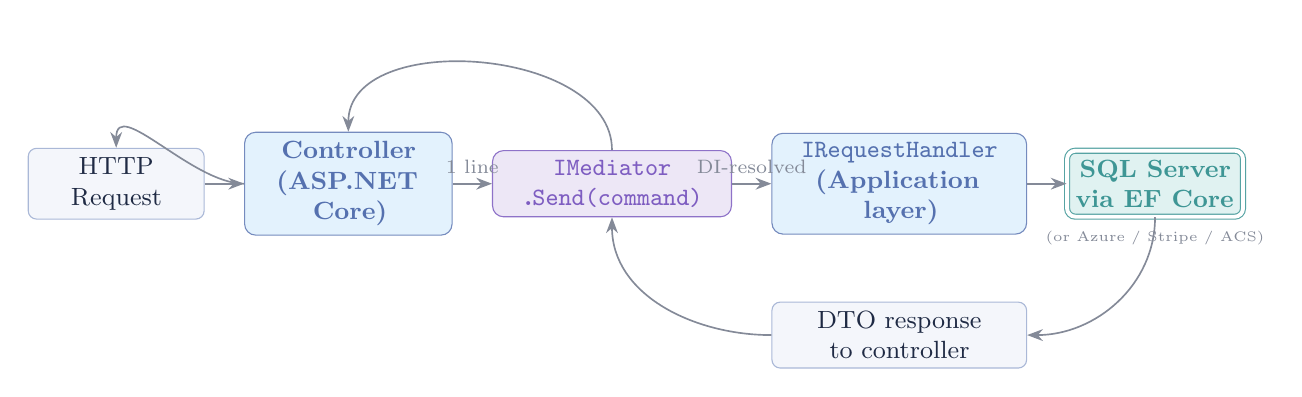
\begin{tikzpicture}[node distance=0.3cm and 0.5cm]
  \node[sbox,text width=2.0cm] (http) {HTTP\\Request};
  \node[pbox,right=0.5cm of http,text width=2.4cm] (ctrl)
    {Controller\\(ASP.NET Core)};
  \node[gbox,right=0.5cm of ctrl,text width=2.8cm] (med)
    {\texttt{IMediator}\\.\texttt{Send(command)}};
  \node[pbox,right=0.5cm of med,text width=3.0cm] (hdlr)
    {\texttt{IRequestHandler}\\(Application layer)};
  \node[dbbox,right=0.5cm of hdlr,text width=2.0cm] (db)
    {SQL Server\\via EF Core};
  \node[sbox,below=0.85cm of hdlr,text width=3.0cm] (resp)
    {DTO response\\to controller};

  \draw[arr] (http) -- (ctrl);
  \draw[arr] (ctrl) -- node[lbl,above] {1 line} (med);
  \draw[arr] (med) -- node[lbl,above] {DI-resolved} (hdlr);
  \draw[arr] (hdlr) -- (db);
  \draw[arr] (db.south) to[out=270,in=0] (resp.east);
  \draw[arr] (resp.west) to[out=180,in=270] (med.south);
  \draw[arr] (med.north) to[out=90,in=90] (ctrl.north);
  \draw[arr] (ctrl.west) to[out=180,in=90] (http.north);

  \node[lbl,below=0.05cm of db] {\tiny (or Azure / Stripe / ACS)};
\end{tikzpicture}
\caption{Every API call is one \texttt{mediator.Send()} --- the controller is
  thin (1--3 lines). All business logic lives in the handler in the Application layer.}
\end{figure}

\subsection{Example: AcceptBookingCommand}

\begin{lstlisting}[language={[Sharp]C},caption={AcceptBookingCommandHandler (condensed)}]
[Auditable(AuditAction.BookingAccepted, "ConsultantBooking",
    TargetIdProperty = nameof(BookingId))]
public sealed record AcceptBookingCommand(Guid BookingId) : IRequest;

public sealed class AcceptBookingCommandHandler : IRequestHandler<AcceptBookingCommand>
{
    public async Task Handle(AcceptBookingCommand request, CancellationToken ct)
    {
        // 1. Load aggregate
        var booking = await context.Bookings
            .Include(b => b.Payment).FirstOrDefaultAsync(..., ct);

        // 2. Stripe capture
        await stripeService.CapturePaymentIntentAsync(...);

        // 3. Provision ACS video room
        var room = await meetingService.CreateRoomAsync(booking.Id, ct);
        booking.MeetingRoomId = room.RoomId;

        // 4. Persist & publish domain event
        await context.SaveChangesAsync(ct);
        await publisher.Publish(new BookingConfirmedEvent(...), ct);
    }
}
\end{lstlisting}

\begin{whybox}
\textbf{Why CQRS?}
\begin{enumerate}
  \item \textbf{Thin controllers} --- controllers become routing-only;
    all business rules live in testable handler classes.
  \item \textbf{Single responsibility} --- each command or query has exactly
    one purpose. Adding a new feature means adding a new handler, not modifying
    an existing service.
  \item \textbf{Audit by decoration} --- \texttt{[Auditable]} is a MediatR
    pipeline behaviour: any command decorated with it automatically creates an
    \texttt{AuditLog} entry before the handler runs.
  \item \textbf{Read/Write separation} --- read queries bypass business-rule
    validation (no unnecessary \texttt{Include}s or domain logic).
\end{enumerate}
\end{whybox}

\subsection{Pipeline Behaviours (Cross-Cutting Concerns)}

MediatR allows middleware-style behaviours that wrap every handler automatically:

\begin{center}
\begin{tabular}{lp{9cm}}
\toprule
\textbf{Behaviour} & \textbf{Effect}\\
\midrule
\texttt{ValidationBehaviour} & Runs FluentValidation before the handler. Throws \texttt{ValidationException} on failure.\\
\texttt{AuditBehaviour} & Writes \texttt{AuditLog} row for commands marked \texttt{[Auditable]}.\\
\texttt{UnhandledExceptionBehaviour} & Catches all handler exceptions, logs them, re-throws.\\
\bottomrule
\end{tabular}
\end{center}

% ═════════════════════════════════════════════════════════════════════════════
\section{Authentication \& Security}
% ═════════════════════════════════════════════════════════════════════════════

\begin{center}
\begin{tabular}{lp{10cm}}
\toprule
\textbf{Mechanism} & \textbf{Detail}\\
\midrule
Identity provider & ASP.NET Core Identity (users, roles, claims)\\
JWT algorithm & \textbf{RS256} (asymmetric) --- private key signs, public key verifies.
  More secure than HS256: the public key can be shared with any verifier.\\
Access token TTL & 15 minutes\\
Refresh token & Opaque token, rotated on every use (old token invalidated).
  Stored in HTTP-only cookie.\\
SSO & Google OAuth 2.0 and Microsoft (Entra ID) via \texttt{ExternalLoginInfo}\\
Roles & \texttt{SuperAdmin}, \texttt{Admin}, \texttt{Student},
        \texttt{Consultant}, \texttt{Company}\\
2FA & TOTP (authenticator app) via ASP.NET Identity \texttt{TwoFactor} flow\\
\bottomrule
\end{tabular}
\end{center}

\begin{figure}[H]
\centering
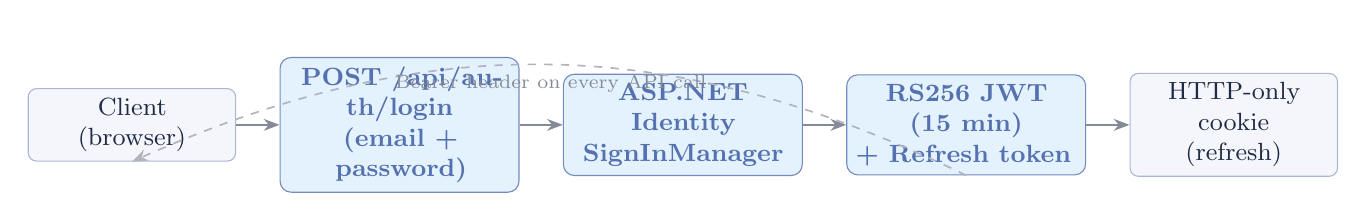
\begin{tikzpicture}[node distance=0.35cm and 0.55cm]
  \node[sbox,text width=2.4cm] (usr) {Client\\(browser)};
  \node[pbox,right=0.55cm of usr,text width=2.8cm] (login)
    {POST /api/auth/login\\(email + password)};
  \node[pbox,right=0.55cm of login,text width=2.8cm] (identity)
    {ASP.NET\\Identity\\SignInManager};
  \node[pbox,right=0.55cm of identity,text width=2.8cm] (jwt)
    {RS256 JWT\\(15 min)\\+ Refresh token};
  \node[sbox,right=0.55cm of jwt,text width=2.4cm] (cookie)
    {HTTP-only\\cookie\\(refresh)};

  \draw[arr] (usr) -- (login);
  \draw[arr] (login) -- (identity);
  \draw[arr] (identity) -- (jwt);
  \draw[arr] (jwt) -- (cookie);
  \draw[arrd] (jwt.south) to[bend right=25]
    node[lbl,below] {Bearer header on every API call} (usr.south);
\end{tikzpicture}
\caption{Login flow. Access token travels in the Authorization header;
  refresh token is stored in an HTTP-only cookie (never accessible to JavaScript).}
\end{figure}

% ═════════════════════════════════════════════════════════════════════════════
\section{Real-Time Communication --- SignalR}
% ═════════════════════════════════════════════════════════════════════════════

Three SignalR hubs provide real-time push to connected clients:

\begin{center}
\begin{tabular}{lll}
\toprule
\textbf{Hub} & \textbf{Events pushed} & \textbf{Used by}\\
\midrule
\texttt{ChatHub} & New message, typing indicator, read receipts & Community DMs\\
\texttt{NotificationHub} & Booking confirmed, payment processed, deadline reminder & All roles\\
\texttt{CommunityHub} & New post reactions, replies, online presence & Community feed\\
\bottomrule
\end{tabular}
\end{center}

\begin{figure}[H]
\centering
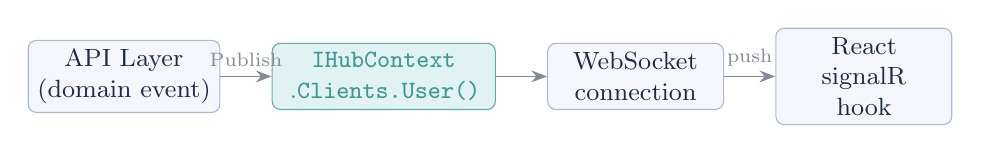
\begin{tikzpicture}[node distance=0.38cm and 0.65cm]
  \node[sbox,text width=2.2cm] (api) {API Layer\\(domain event)};
  \node[tbox,right=0.65cm of api,text width=2.6cm] (hub)
    {\texttt{IHubContext}\\.\texttt{Clients.User()}};
  \node[sbox,text width=2.0cm,right=0.65cm of hub] (ws)
    {WebSocket\\connection};
  \node[sbox,text width=2.0cm,right=0.65cm of ws] (client)
    {React\\signalR\\hook};

  \draw[arr] (api) -- node[lbl,above] {Publish} (hub);
  \draw[arr] (hub) -- (ws);
  \draw[arr] (ws) -- node[lbl,above] {push} (client);
\end{tikzpicture}
\caption{Real-time push: a domain event triggers \texttt{IHubContext.Clients.User(id).SendAsync(...)}.
  The client's \texttt{useSignalR} hook updates React state immediately.}
\end{figure}

% ═════════════════════════════════════════════════════════════════════════════
\section{Video Meeting --- PB-006 (Azure Communication Services)}
% ═════════════════════════════════════════════════════════════════════════════

\begin{keybox}{What it is}
A full in-browser video call between student and consultant, powered by
\textbf{Azure Communication Services (ACS)}.
The meeting is automatically created when a booking is confirmed
and recorded to Azure Blob Storage.
\end{keybox}

\subsection{Why Azure Communication Services?}

\begin{center}
\begin{tabular}{lp{5.5cm}p{5.5cm}}
\toprule
\textbf{Option} & \textbf{Pros} & \textbf{Cons \& why rejected}\\
\midrule
Jitsi (self-hosted) & Free, open-source & Requires VM + ops; no built-in recording\\
Twilio & Mature, well-documented & Higher cost, US-centric data residency\\
\textbf{ACS} & Azure ecosystem, SLA, built-in recording, PII compliance & Slightly steeper SDK learning curve\\
\bottomrule
\end{tabular}
\end{center}

\subsection{Complete Video Meeting Flow (12 Steps)}

\begin{figure}[H]
\centering
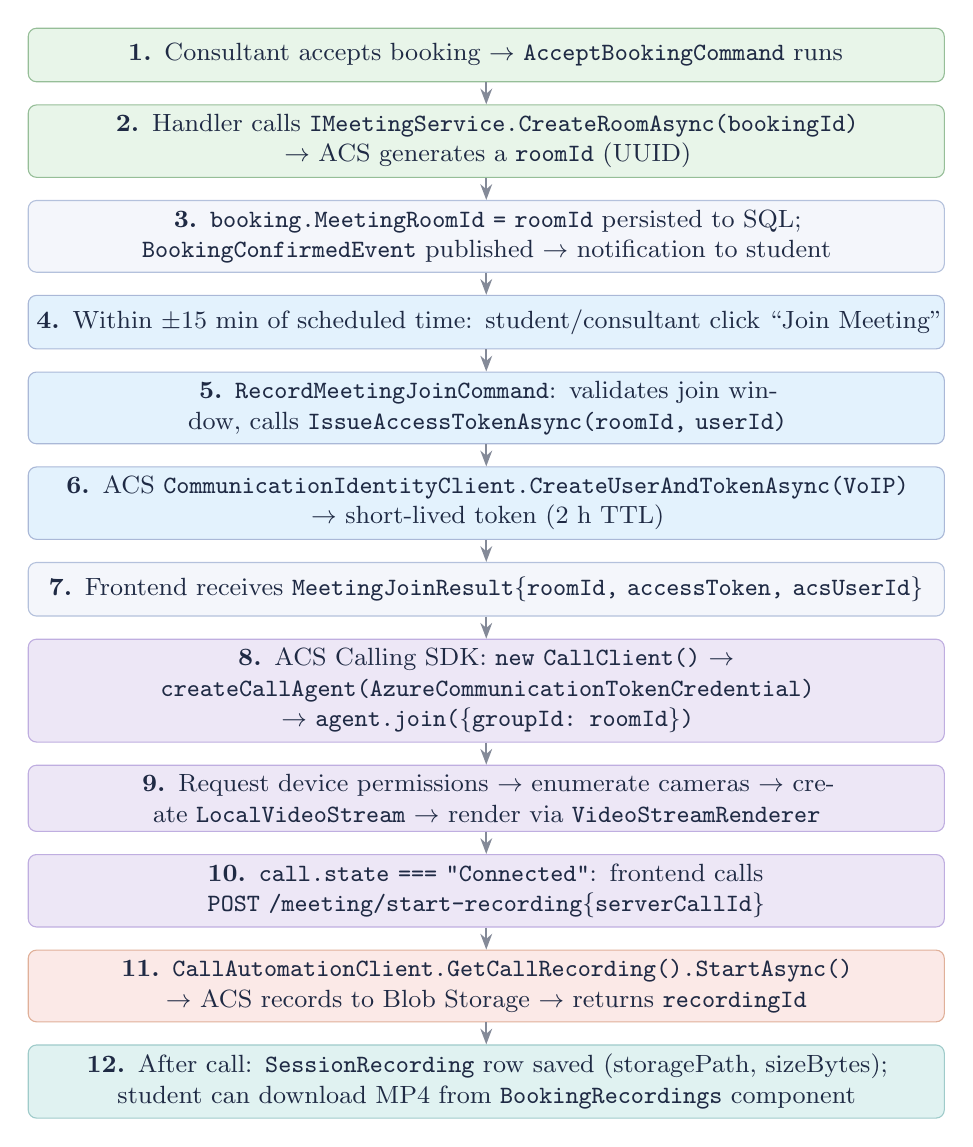
\begin{tikzpicture}[node distance=0.3cm]

  \node[wbox,fill=spLightGreen,draw=spWhy!50] (s1)
    {\textbf{1.} Consultant accepts booking $\rightarrow$
     \texttt{AcceptBookingCommand} runs};

  \node[wbox,below=0.28cm of s1,fill=spLightGreen,draw=spWhy!50] (s2)
    {\textbf{2.} Handler calls \texttt{IMeetingService.CreateRoomAsync(bookingId)}
     $\rightarrow$ ACS generates a \texttt{roomId} (UUID)};

  \node[wbox,below=0.28cm of s2] (s3)
    {\textbf{3.} \texttt{booking.MeetingRoomId = roomId} persisted to SQL;
     \texttt{BookingConfirmedEvent} published $\rightarrow$ notification to student};

  \node[wbox,below=0.28cm of s3,fill=spLightBlue,draw=spPrimary!40] (s4)
    {\textbf{4.} Within $\pm15$ min of scheduled time: student/consultant click
     ``Join Meeting''};

  \node[wbox,below=0.28cm of s4,fill=spLightBlue,draw=spPrimary!40] (s5)
    {\textbf{5.} \texttt{RecordMeetingJoinCommand}: validates join window,
     calls \texttt{IssueAccessTokenAsync(roomId, userId)}};

  \node[wbox,below=0.28cm of s5,fill=spLightBlue,draw=spPrimary!40] (s6)
    {\textbf{6.} ACS \texttt{CommunicationIdentityClient.CreateUserAndTokenAsync(VoIP)}
     $\rightarrow$ short-lived token (2 h TTL)};

  \node[wbox,below=0.28cm of s6] (s7)
    {\textbf{7.} Frontend receives \texttt{MeetingJoinResult\{roomId, accessToken, acsUserId\}}};

  \node[wbox,below=0.28cm of s7,fill=spLightPurple,draw=spQA!40] (s8)
    {\textbf{8.} ACS Calling SDK: \texttt{new CallClient()} $\rightarrow$
     \texttt{createCallAgent(AzureCommunicationTokenCredential)} $\rightarrow$
     \texttt{agent.join(\{groupId: roomId\})}};

  \node[wbox,below=0.28cm of s8,fill=spLightPurple,draw=spQA!40] (s9)
    {\textbf{9.} Request device permissions $\rightarrow$ enumerate cameras
     $\rightarrow$ create \texttt{LocalVideoStream} $\rightarrow$
     render via \texttt{VideoStreamRenderer}};

  \node[wbox,below=0.28cm of s9,fill=spLightPurple,draw=spQA!40] (s10)
    {\textbf{10.} \texttt{call.state === "Connected"}: frontend calls
     \texttt{POST /meeting/start-recording\{serverCallId\}}};

  \node[wbox,below=0.28cm of s10,fill=spLightOrange,draw=spSec!40] (s11)
    {\textbf{11.} \texttt{CallAutomationClient.GetCallRecording().StartAsync()} $\rightarrow$
     ACS records to Blob Storage $\rightarrow$
     returns \texttt{recordingId}};

  \node[wbox,below=0.28cm of s11,fill=spLightTeal,draw=spAccent!40] (s12)
    {\textbf{12.} After call: \texttt{SessionRecording} row saved (storagePath, sizeBytes);
     student can download MP4 from \texttt{BookingRecordings} component};

  \foreach \from/\to in {s1/s2,s2/s3,s3/s4,s4/s5,s5/s6,s6/s7,s7/s8,s8/s9,s9/s10,s10/s11,s11/s12}
    \draw[arr] (\from) -- (\to);

\end{tikzpicture}
\caption{Complete video meeting lifecycle.
  \colorbox{spLightGreen!60}{Green} = booking confirmation phase.
  \colorbox{spLightBlue!60}{Blue} = join validation.
  \colorbox{spLightPurple!60}{Purple} = ACS SDK in frontend.
  \colorbox{spLightOrange!60}{Orange} = server-side recording.
  \colorbox{spLightTeal!60}{Teal} = post-session storage.}
\end{figure}

\subsection{Key Design Decisions}

\begin{center}
\begin{tabular}{lp{10.5cm}}
\toprule
\textbf{Decision} & \textbf{Rationale}\\
\midrule
Join window $\pm15$ min &
  Prevents students from squatting in rooms hours before the session.
  Controlled by \texttt{JoinOpensBefore = JoinClosesAfter = TimeSpan.FromMinutes(15)}.\\[4pt]
Lazy room provisioning &
  \texttt{MeetingRoomId} is set at booking acceptance, but if it is missing
  (legacy records), a new room is created at join time automatically.\\[4pt]
Short-lived token (2 h) &
  ACS tokens expire after 2 h. For sessions exceeding this,
  the frontend would need to refresh --- acceptable for a 60-min max session.\\[4pt]
Stub implementation &
  \texttt{StubMeetingService} is injected in development.
  \texttt{join.provider === "Stub"} triggers a clear error message on the
  frontend: ``Video not configured --- contact admin.''\\[4pt]
Attendance tracking &
  \texttt{StudentJoinedAt} and \texttt{ConsultantJoinedAt} are set on first join.
  Used by the no-show detection job (FR-217).\\
\bottomrule
\end{tabular}
\end{center}

\subsection{Frontend --- ACS Calling SDK Integration}

\begin{lstlisting}[caption={Meeting.tsx --- SDK bootstrap (condensed)}]
// 1. Get credentials from server
const join = await meetingsApi.join(bookingId);

// 2. Init ACS calling client + agent
const callClient = new CallClient();
const credential = new AzureCommunicationTokenCredential(join.accessToken);
const agent = await callClient.createCallAgent(credential, { displayName });

// 3. Device permissions + local camera
const deviceManager = await callClient.getDeviceManager();
await deviceManager.askDevicePermission({ video: true, audio: true });
const cameras = await deviceManager.getCameras();
const localStream = new LocalVideoStream(cameras[0]);

// 4. Join the group call
const call = agent.join(
  { groupId: join.roomId },
  { videoOptions: { localVideoStreams: [localStream] },
    audioOptions: { muted: false } },
);

// 5. Render local video
const view = await new VideoStreamRenderer(localStream).createView();
localVideoRef.current.replaceChildren(view.target);

// 6. Watch for remote participants
call.on("remoteParticipantsUpdated", (e) => {
  e.added.forEach(watchParticipant);
});

// 7. Start recording once connected
call.on("stateChanged", async () => {
  if (call.state === "Connected") {
    const serverCallId = await call.info.getServerCallId();
    await meetingsApi.startRecording(bookingId, serverCallId);
    setRecording(true);
  }
});
\end{lstlisting}

% ═════════════════════════════════════════════════════════════════════════════
\section{Background Jobs --- Hangfire}
% ═════════════════════════════════════════════════════════════════════════════

Five recurring jobs run on the application server:

\begin{center}
\begin{tabular}{lll}
\toprule
\textbf{Job} & \textbf{Schedule} & \textbf{Action}\\
\midrule
KB Nightly Rebuild & Nightly 02:00 UTC & Incremental knowledge base rebuild\\
Deadline Reminder & Daily 08:00 UTC & Notifies students: 7-day + 1-day alerts\\
Payment Settlement & Every 15 min & Confirms captured Stripe payments\\
No-Show Detection & Hourly & Marks bookings where no participant joined\\
Analytics Sync & Nightly 03:00 UTC & Triggers ADF pipeline (Bronze refresh)\\
\bottomrule
\end{tabular}
\end{center}

% ═════════════════════════════════════════════════════════════════════════════
\section{Analytics Data Pipeline (PB-015 -- PB-018)}
% ═════════════════════════════════════════════════════════════════════════════

\begin{figure}[H]
\centering
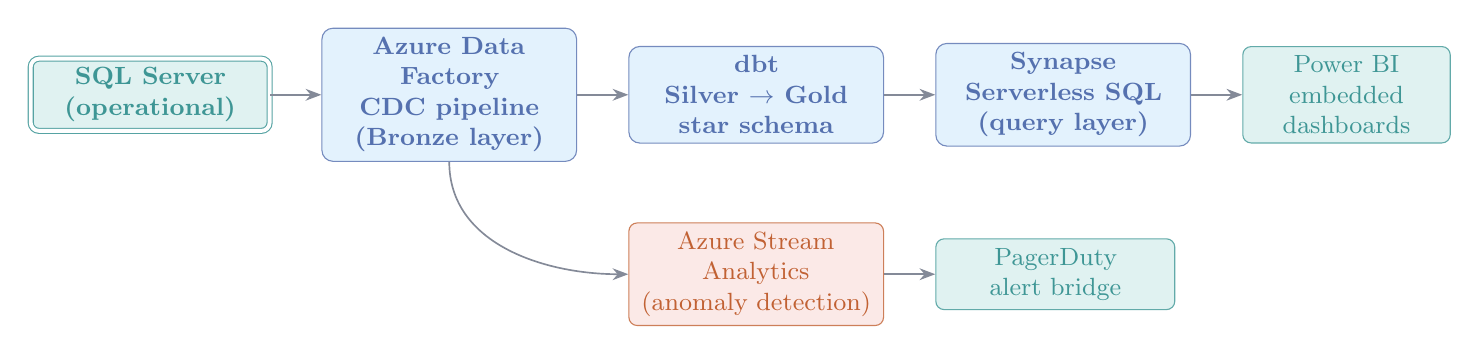
\begin{tikzpicture}[node distance=0.38cm and 0.55cm]
  \node[dbbox,text width=2.8cm] (sql) {SQL Server\\(operational)};
  \node[pbox,right=0.65cm of sql,text width=3.0cm] (adf)
    {Azure Data Factory\\CDC pipeline\\(Bronze layer)};
  \node[pbox,right=0.65cm of adf,text width=3.0cm] (dbt)
    {dbt\\Silver $\rightarrow$ Gold\\star schema};
  \node[pbox,right=0.65cm of dbt,text width=3.0cm] (syn)
    {Synapse\\Serverless SQL\\(query layer)};
  \node[tbox,right=0.65cm of syn,text width=2.4cm] (pbi)
    {Power BI\\embedded\\dashboards};

  % Stream analytics branch
  \node[fbox,below=1.0cm of dbt,text width=3.0cm] (sa)
    {Azure Stream\\Analytics\\(anomaly detection)};
  \node[tbox,right=0.65cm of sa,text width=2.8cm] (pd)
    {PagerDuty\\alert bridge};

  \draw[arr] (sql) -- (adf);
  \draw[arr] (adf) -- (dbt);
  \draw[arr] (dbt) -- (syn);
  \draw[arr] (syn) -- (pbi);
  \draw[arr] (adf.south) to[out=270,in=180] (sa.west);
  \draw[arr] (sa) -- (pd);
\end{tikzpicture}
\caption{Analytics pipeline. CDC from SQL Server flows through ADF into the Bronze
  zone; dbt transforms to a Gold star schema (fact + dimension tables); Synapse
  Serverless exposes views to Power BI. A parallel Stream Analytics branch detects
  anomalies in real time and fires PagerDuty alerts.}
\end{figure}

% ═════════════════════════════════════════════════════════════════════════════
\section{Mahmoud's Modules --- Deep Dive}
% ═════════════════════════════════════════════════════════════════════════════

As team lead and architect, Mahmoud owns 6 of the 18 PB epics:

\begin{center}
\begin{tabular}{clp{9.0cm}}
\toprule
\textbf{PB} & \textbf{Module} & \textbf{Key deliverables}\\
\midrule
\textbf{008} & AI Features &
  RAG chatbot, recommendation scoring, eligibility check,
  KnowledgeBase indexer, fine-tuning dataset,
  admin KB management page, \texttt{AiInteraction} entity\\[3pt]
\textbf{011} & Admin Portal &
  \texttt{AdminLayout} with 17-item navigation, admin dashboard (revenue widget,
  user growth chart), admin management pages for every entity\\[3pt]
\textbf{012} & Audit \& Compliance &
  \texttt{AuditBehaviour} (MediatR pipeline), \texttt{AuditLog} table,
  admin audit log viewer with full-text search,
  PII redaction sampling for AI chat responses\\[3pt]
\textbf{016} & Data Warehouse &
  Azure Data Factory CDC pipelines (Bronze),
  dbt project (Silver \& Gold star schema),
  Synapse Serverless views,
  reverse-ETL from Gold back to operational DB\\[3pt]
\textbf{017} & AI Economy &
  Daily cost tracking per user \& provider,
  \texttt{DailyCostLimitUsd} hard cap enforcement,
  recommendation click-through rate (CTR) tracking,
  admin AI cost dashboard\\[3pt]
\textbf{018} & Real-time Streaming &
  Azure Stream Analytics job (payment anomalies + KB-rebuild triggers),
  PagerDuty webhook bridge,
  real-time Stripe event processing\\
\bottomrule
\end{tabular}
\end{center}

\subsection{PB-008 AI --- Feature Ownership Summary}

See companion document \textit{06-ai-architecture-deep-dive.pdf} for full detail.
Key summary:

\begin{itemize}
  \item \textbf{Chatbot} (\texttt{AzureOpenAiService.AskAsync}): Standard RAG,
    5-doc context, GPT-4o-mini, 3-level fallback to \texttt{LocalAiService}.
  \item \textbf{Recommendations} (\texttt{LocalAiService}): Deterministic scoring
    (Level 30 + Field 40 + Country 25 + Bonus 5), cached in \texttt{AiInteraction},
    live re-hydration on read.
  \item \textbf{Eligibility} (\texttt{LocalAiService}): 3-criterion profile match
    $\rightarrow$ Eligible / PartiallyEligible / NotEligible verdict.
  \item \textbf{Admin KB page}: 4-button control panel (rebuild, force rebuild, import, JSONL export).
\end{itemize}

\subsection{PB-012 Audit --- How Auditing Works}

\begin{lstlisting}[language={[Sharp]C},caption={Any command decorated with [Auditable] is automatically audited}]
// In any Command record:
[Auditable(AuditAction.ScholarshipDeleted, "Scholarship",
    TargetIdProperty = nameof(ScholarshipId))]
public sealed record DeleteScholarshipCommand(Guid ScholarshipId) : IRequest;

// AuditBehaviour (registered as MediatR pipeline behaviour) intercepts it:
// 1. Reads [Auditable] attribute before handler runs
// 2. After handler succeeds: inserts AuditLog row
//    { UserId, Action, EntityType, EntityId, Timestamp, IpAddress }
// 3. Admin can query /api/admin/audit-logs with full-text search
\end{lstlisting}

% ═════════════════════════════════════════════════════════════════════════════
\section{Defence Presentation Flow}
% ═════════════════════════════════════════════════════════════════════════════

\begin{defencebox}
This section gives the recommended order and talking points for presenting
ScholarPath to the academic committee. Each block has a suggested time budget.
\end{defencebox}

\begin{figure}[H]
\centering
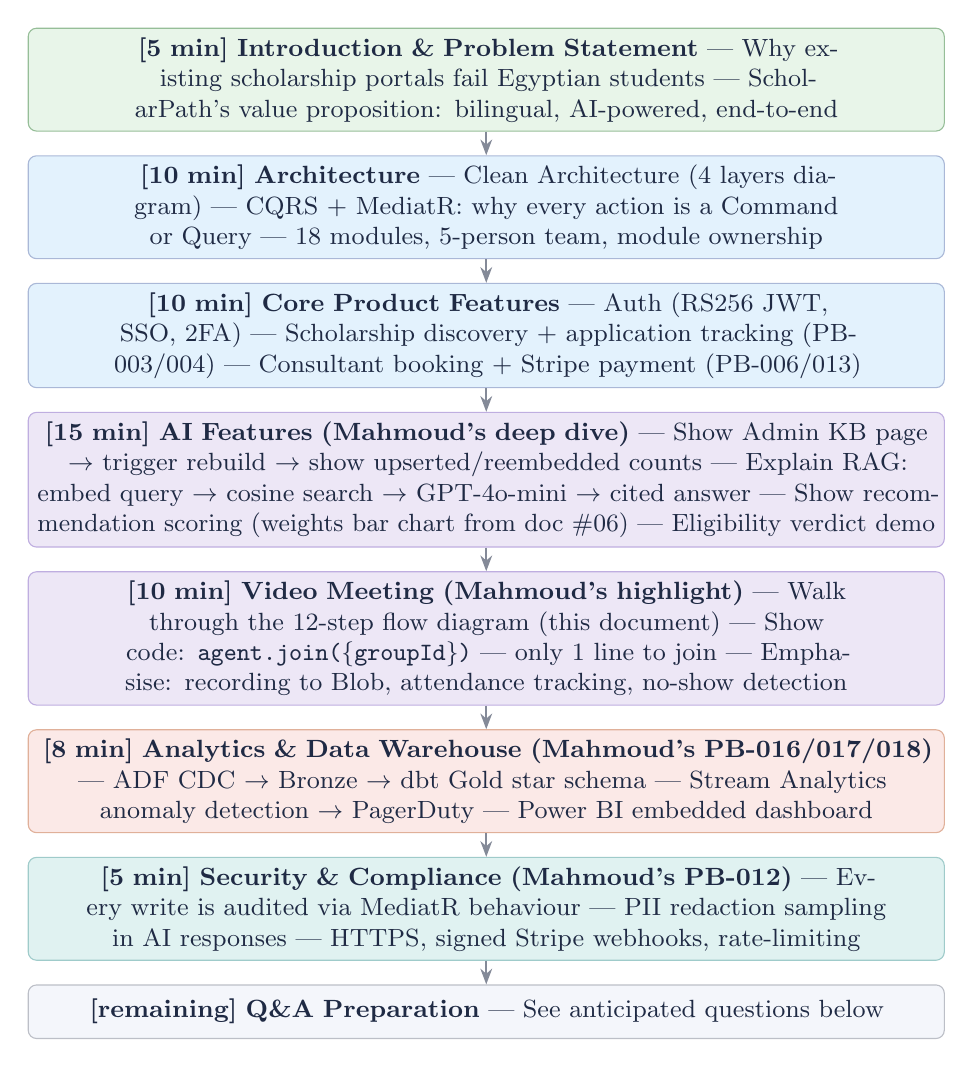
\begin{tikzpicture}[node distance=0.32cm]

  \node[wbox,fill=spLightGreen,draw=spWhy!50] (d1)
    {\textbf{[5 min] Introduction \& Problem Statement}
     --- Why existing scholarship portals fail Egyptian students
     --- ScholarPath's value proposition: bilingual, AI-powered, end-to-end};

  \node[wbox,below=0.3cm of d1,fill=spLightBlue,draw=spPrimary!40] (d2)
    {\textbf{[10 min] Architecture}
     --- Clean Architecture (4 layers diagram)
     --- CQRS + MediatR: why every action is a Command or Query
     --- 18 modules, 5-person team, module ownership};

  \node[wbox,below=0.3cm of d2,fill=spLightBlue,draw=spPrimary!40] (d3)
    {\textbf{[10 min] Core Product Features}
     --- Auth (RS256 JWT, SSO, 2FA)
     --- Scholarship discovery + application tracking (PB-003/004)
     --- Consultant booking + Stripe payment (PB-006/013)};

  \node[wbox,below=0.3cm of d3,fill=spLightPurple,draw=spQA!40] (d4)
    {\textbf{[15 min] AI Features (Mahmoud's deep dive)}
     --- Show Admin KB page $\rightarrow$ trigger rebuild $\rightarrow$ show upserted/reembedded counts
     --- Explain RAG: embed query $\rightarrow$ cosine search $\rightarrow$ GPT-4o-mini $\rightarrow$ cited answer
     --- Show recommendation scoring (weights bar chart from doc \#06)
     --- Eligibility verdict demo};

  \node[wbox,below=0.3cm of d4,fill=spLightPurple,draw=spQA!40] (d5)
    {\textbf{[10 min] Video Meeting (Mahmoud's highlight)}
     --- Walk through the 12-step flow diagram (this document)
     --- Show code: \texttt{agent.join(\{groupId\})} --- only 1 line to join
     --- Emphasise: recording to Blob, attendance tracking, no-show detection};

  \node[wbox,below=0.3cm of d5,fill=spLightOrange,draw=spSec!40] (d6)
    {\textbf{[8 min] Analytics \& Data Warehouse (Mahmoud's PB-016/017/018)}
     --- ADF CDC $\rightarrow$ Bronze $\rightarrow$ dbt Gold star schema
     --- Stream Analytics anomaly detection $\rightarrow$ PagerDuty
     --- Power BI embedded dashboard};

  \node[wbox,below=0.3cm of d6,fill=spLightTeal,draw=spAccent!40] (d7)
    {\textbf{[5 min] Security \& Compliance (Mahmoud's PB-012)}
     --- Every write is audited via MediatR behaviour
     --- PII redaction sampling in AI responses
     --- HTTPS, signed Stripe webhooks, rate-limiting};

  \node[wbox,below=0.3cm of d7,fill=spGrayBg,draw=spInk!30] (d8)
    {\textbf{[remaining] Q\&A Preparation}
     --- See anticipated questions below};

  \foreach \from/\to in {d1/d2,d2/d3,d3/d4,d4/d5,d5/d6,d6/d7,d7/d8}
    \draw[arr] (\from) -- (\to);

\end{tikzpicture}
\caption{Recommended defence presentation order. Total: $\approx$63 minutes with buffer
  for questions between sections.}
\end{figure}

\subsection{Anticipated Committee Questions --- and Answers}

\begin{center}
\begin{tabularx}{\linewidth}{p{5.8cm}X}
\toprule
\textbf{Question} & \textbf{Answer}\\
\midrule
``Why Clean Architecture instead of a simple layered architecture?'' &
  Clean Architecture enforces dependency inversion --- the domain has zero
  knowledge of EF Core or Azure. This means we can swap the database (or any
  service) without touching business logic. We verified this by injecting a
  \texttt{Stub} implementation for all external services (ACS, Stripe, Azure) in tests.\\[4pt]
``Why CQRS for a graduation project? Is it overkill?'' &
  The project has 211 FRs across 5 developers. CQRS enforced clear
  ownership boundaries --- each handler is a single C\# file owned by one person.
  Without it, a shared service class would have caused merge conflicts on every sprint.
  MediatR also gave us cross-cutting audit behaviour for free.\\[4pt]
``Why not use a vector database?'' &
  At 692 documents, a full in-memory cosine scan completes in $<10$\,ms.
  A vector DB would add a network hop and operational cost with no accuracy benefit.
  The migration path exists: swap \texttt{KnowledgeRetriever} with
  a Qdrant or pgvector implementation.\\[4pt]
``Is the AI hallucinating?'' &
  The system prompt prohibits fabrication, and the answer must cite
  the numbered context block. The RAG context is grounded in the live database;
  if no document scores above 0.6, the local fallback gives a generic answer
  rather than guessing.\\[4pt]
``Why Azure ACS for video and not Jitsi?'' &
  Jitsi requires a self-hosted VM with operational overhead and has no
  built-in recording API. ACS provides a managed, PII-compliant recording
  pipeline and integrates natively with the rest of our Azure stack.\\[4pt]
``How does billing work for consultants?'' &
  Stripe PaymentIntents with manual capture. The student's card is authorised
  at booking time; capture happens only when the consultant accepts.
  Platform profit share is calculated at the handler level (Stripe Transfer).\\[4pt]
``What happens if Azure OpenAI is down?'' &
  Three-level fallback: (1) config missing $\rightarrow$ local; (2) HTTP error on
  embedding call $\rightarrow$ local; (3) GPT call fails $\rightarrow$ local.
  \texttt{LocalAiService.AskAsync} runs the same RAG retrieval without GPT, then
  falls back to a keyword router. Users always get a response.\\
\bottomrule
\end{tabularx}
\end{center}

% ═════════════════════════════════════════════════════════════════════════════
\section{Summary --- What Makes ScholarPath Distinctive}
% ═════════════════════════════════════════════════════════════════════════════

\begin{keybox}{Three differentiators}
\textbf{1. Spec-driven development} --- every PR references an FR-xxx or US-xxx.
Every entity has a migration. Every audit-relevant command has
\texttt{[Auditable]}. 211 FRs fully implemented.

\medskip
\textbf{2. Production-grade AI at zero marginal cost} --- RAG chatbot + deterministic
recommendations + eligibility checking, with a three-level fallback so the system
degrades gracefully under any Azure failure. Daily cost cap prevents runaway billing.

\medskip
\textbf{3. End-to-end video infrastructure} --- ACS room provisioning, short-lived token
issuance, client-side ACS Calling SDK, server-side recording, Blob storage, and MP4
download --- all wired together in 12 steps with attendance tracking and no-show detection.
\end{keybox}

\end{document}
